\documentclass[tikz]{article}

% Packages
\usepackage[utf8]{inputenc} % Core latex bundle 
\usepackage[a4paper, total={6in, 9in}]{geometry} % Customize document dimensions and formats
\usepackage{changepage} % Customize page layout in middle of document
\usepackage[table]{xcolor} % Add color to tables
\usepackage{standalone} % Add figures and tables from other files
\usepackage{import} % Import glossary
\usepackage{graphics} % General color and formats
\usepackage{url} % URL formatting
\usepackage{breakurl} % URL formatting
\usepackage{enumitem} % Format list spacing 
\usepackage[hang]{footmisc} % Footnote margins
\usepackage{hyperref} % References
\usepackage{mathtools} % Useful tools for mathematical typesetting and replaces amsmath
\usepackage{amssymb,bm} % Math symbols
\usepackage{svg} % SVG
\usepackage{tikz} % Making charts
\usepackage{array,boldline,multirow,float,booktabs} % Added to make tables
\usepackage{stackengine} % Customize row heights
\usepackage{hhline} % Add double lines to table
\usepackage{multicol} % Two column lists
\usepackage{nicematrix} % Put table lines after color
\usepackage{wrapfig} % Wrap figures in text
\usepackage{tocloft,titletoc} % TOC package
\usepackage{titlesec} % Section spacing

% Copyright 2017 Sergei Tikhomirov, MIT License
% https://github.com/s-tikhomirov/solidity-latex-highlighting/

\usepackage{listings, xcolor}

\definecolor{verylightgray}{rgb}{.97,.97,.97}

\lstdefinelanguage{Solidity}{
	keywords=[1]{anonymous, assembly, assert, balance, break, call, callcode, case, catch, class, constant, continue, constructor, contract, debugger, default, delegatecall, delete, do, else, emit, event, experimental, export, external, false, finally, for, function, gas, if, implements, import, in, indexed, instanceof, interface, internal, is, length, library, log0, log1, log2, log3, log4, memory, modifier, new, payable, pragma, private, protected, public, pure, push, require, return, returns, revert, selfdestruct, send, solidity, storage, struct, suicide, super, switch, then, this, throw, transfer, true, try, typeof, using, value, view, while, with, addmod, ecrecover, keccak256, mulmod, ripemd160, sha256, sha3}, % generic keywords including crypto operations
	keywordstyle=[1]\color{blue}\bfseries,
	keywords=[2]{address, bool, byte, bytes, bytes1, bytes2, bytes3, bytes4, bytes5, bytes6, bytes7, bytes8, bytes9, bytes10, bytes11, bytes12, bytes13, bytes14, bytes15, bytes16, bytes17, bytes18, bytes19, bytes20, bytes21, bytes22, bytes23, bytes24, bytes25, bytes26, bytes27, bytes28, bytes29, bytes30, bytes31, bytes32, enum, int, int8, int16, int24, int32, int40, int48, int56, int64, int72, int80, int88, int96, int104, int112, int120, int128, int136, int144, int152, int160, int168, int176, int184, int192, int200, int208, int216, int224, int232, int240, int248, int256, mapping, string, uint, uint8, uint16, uint24, uint32, uint40, uint48, uint56, uint64, uint72, uint80, uint88, uint96, uint104, uint112, uint120, uint128, uint136, uint144, uint152, uint160, uint168, uint176, uint184, uint192, uint200, uint208, uint216, uint224, uint232, uint240, uint248, uint256, var, void, ether, finney, szabo, wei, days, hours, minutes, seconds, weeks, years},	% types; money and time units
	keywordstyle=[2]\color{teal}\bfseries,
	keywords=[3]{block, blockhash, coinbase, difficulty, gaslimit, number, timestamp, msg, data, gas, sender, sig, value, now, tx, gasprice, origin},	% environment variables
	keywordstyle=[3]\color{violet}\bfseries,
	identifierstyle=\color{black},
	sensitive=false,
	comment=[l]{//},
	morecomment=[s]{/*}{*/},
	commentstyle=\color{gray}\ttfamily,
	stringstyle=\color{red}\ttfamily,
	morestring=[b]',
	morestring=[b]"
}

\lstset{
	language=Solidity,
	backgroundcolor=\color{verylightgray},
	extendedchars=true,
	basicstyle=\footnotesize\ttfamily,
	showstringspaces=false,
	showspaces=false,
	numbers=left,
	numberstyle=\footnotesize,
	numbersep=9pt,
	tabsize=2,
	breaklines=true,
	showtabs=false,
	captionpos=b
}	% https://github.com/s-tikhomirov/solidity-latex-highlighting

% Paper formatting
\newlength\LabelWidth
\setlength\parindent{0pt}
\setlength{\parskip}{1em}

% Section spacing
\titlespacing*{\section}
  {0pt}{0.6\baselineskip}{0.6\baselineskip} % Modify section spacing - first \baselineskip is spacing before, second is spacing after the section
\titlespacing*{\subsection}
  {0pt}{0.6\baselineskip}{0.6\baselineskip} % Modify subsection spacing 
\titlespacing*{\subsubsection}
  {0pt}{0.6\baselineskip}{0.6\baselineskip} % Modify subsubsection spacing

% String formats
\newcommand{\code}[1]{\texttt{#1}}
\newcommand{\term}[1]{\textsl{#1}}

% Paper margins
\def\changemargin#1#2{\list{}{\rightmargin#2\leftmargin#1}\item[]}
\let\endchangemargin=\endlist

% Table of contents
\renewcommand{\contentsname}{Table of Contents}
\renewcommand{\cfttoctitlefont}{\Large\bfseries} % TOC title size
\renewcommand{\cftsecleader}{\cftdotfill{\cftdotsep}} % Add dots in TOC to sections
\renewcommand{\cftsecpagefont}{} % Remove \bfseries from section titles' page in TOC

% Section
\renewcommand*{\cftsecnumwidth}{2em} % Increase space section from numbers on left

% Subsection
\cftsetindents{subsection}{1em}{3em} % space between numbers and toc subsections
\setlength{\cftsubsecindent}{2.5em} % subsection number spacing from left
\setlength{\cftbeforesubsecskip}{3pt} % Messes with subsection TOC length was 3pt

% Subsubsection
\cftsetindents{subsubsection}{1em}{4em} % space between numbers and toc subsubsections
\setlength{\cftsubsubsecindent}{5.5em} % subsubsection number spacing from leftindent
\setlength{\cftbeforesubsubsecskip}{3pt} % Messes with subsubsection TOC length was 3pt

% paragraph section
\setcounter{secnumdepth}{4}
\setcounter{tocdepth}{4}

\cftsetindents{paragraph}{1em}{5em} % space between numbers and toc paragraph
\setlength{\cftparaindent}{9.5em} % paragraph number spacing from leftindent
\setlength{\cftbeforeparaskip}{3pt} % Messes with paragraph TOC length was 3pt

% indent after paragraph section
\titleformat{\paragraph}
{\normalfont\normalsize\bfseries}{\theparagraph}{1em}{}
\titlespacing*{\paragraph}
{0pt}{3.25ex plus 1ex minus .2ex}{1.5ex plus .2ex}

% Abstract
% Make abstract justified
\makeatletter
\newcommand{\justified}{
  \rightskip\z@skip
  \leftskip\z@skip}
\makeatother

% Format and size abstract
\makeatletter
\renewenvironment{abstract}{
    \if@twocolumn
      \section*{\abstractname}
    \else 
      \begin{center}
        {\bfseries \large\abstractname\vspace{\z@}} % Bolds abstract name
      \end{center}
      \quotation
    \fi}
    {\if@twocolumn\else\endquotation\fi}
\makeatother

% Delimiters
\DeclarePairedDelimiter\floor{\lfloor}{\rfloor} % Define paired delimiter for floor function
\DeclarePairedDelimiter{\ceil}{\lceil}{\rceil} % Define paired delimiter for ceiling function

% Hyperlinks
\hypersetup{
    colorlinks=true,
    linkcolor=black,
    filecolor=blue,
    urlcolor=black,
}
\urlstyle{same}

% Footnotes
\newcommand{\fref}[1]{\footnote{\href{http://#1}{#1}}}
\setlength{\footnotemargin}{8mm} % Spacing between footnote number and body

% Include tables
\makeatletter
\newcommand{\includetable}[1]{%
  \@ifundefined{tablepath}{%
    \InputIfFileExists{#1}{}{}%
  }{%
    \InputIfFileExists{\tablepath/#1}{}{\InputIfFileExists{#1}{}{}}%
  }
}
\makeatother  

% Table formatting commands
\newcolumntype{Q}{ >{\centering\arraybackslash} m{2.4cm} } % (Figure 5 and 11 - col width)
\newcolumntype{S}{ >{\centering\arraybackslash} m{5.27cm} } % (Figure 12 - col width double)
\newcommand\xrowht[2][0]{\addstackgap[.5\dimexpr#2\relax]{\vphantom{#1}}} % Set row height for tables
\newcommand{\rowh}[1]{\xrowht{40pt}} % Command to set row height for cell with 3 rows
\newcommand{\rowm}[1]{\xrowht{26.667pt}} % Command to set row height for cell with 2 rows
\newcommand{\rows}[1]{\xrowht{13.333pt}} % Command to set row height for cell with 1 rows

% Symbols
\newcommand{\PipelineCover}{\includesvg[scale=3.0]{./logos/pipeline.svg}} % Logo on cover page

% List Key
\SetEnumitemKey{midsep}{topsep=0pt, itemsep=3pt} % Itemize key

% File paths
\newcommand{\tablepath}{figures} % Tables file path
\graphicspath{{figures/}} % Figures file path

%%%%%%%   Begin Document   %%%%%%%
\begin{document}
\pagenumbering{arabic} % Start page numbering style
\thispagestyle{empty} % Hide page numbering
\begin{titlepage}
    \begin{center}
        \vspace*{-0.1cm}
        \begin{changemargin}{-0.25cm}{-0.25cm}
        \centering % added to center title
        \textbf{\Large{Pipeline \& Depot: Dance Through the EVM in 1 Transaction}}
        \end{changemargin}
        \begin{center}
        \PipelineCover
        \end{center}
        \vspace{-0.1cm}

        \begin{center}
            \begin{tabular}{>{\centering\arraybackslash}p{5cm} >{\centering\arraybackslash}p{5cm}}
                \large{Publius} & \large{Silo Chad} \\
                \href{mailto:beanstalk.publius@protonmail.com}{\normalsize{beanstalk.publius@protonmail.com}} & \href{mailto:silochad@protonmail.com}{\normalsize{silochad@protonmail.com}}
            \end{tabular}
        \end{center}
        
        \vspace{-0.25cm}
        \normalsize{\href{https://evmpipeline.org/}{evmpipeline.org}}
        
        \vspace{0.2cm}
        \footnotesize{Published:} \normalsize{November 16, 2022}
        
        \vspace{-0.25cm}
        \footnotesize{Modified:} \normalsize{November 17, 2023}
        
        \vspace{-0.25cm}
        \footnotesize{Whitepaper Version:} {\normalsize{1.0.4}}
        
        \vspace{-0.25cm}
        \footnotesize{Code Version:} {\normalsize{1.0.1}}{\fref{github.com/BeanstalkFarms/Pipeline}}

        \vspace{0.0cm}
        \flushleft{\normalsize{\term{“Leave nothing for to-morrow which can be done to-day.”}}}
        
        \normalsize{\hspace{2.5em}- The Collected Works of Abraham Lincoln edited by Roy P. Basler, Volume II, “Notes for a Law Lecture” (July 1, 1850?), p. 81}\fref{quod.lib.umich.edu/l/lincoln/lincoln2/1:134?rgn=div1;view=fulltext}

        %% new link: https://quod.lib.umich.edu/l/lincoln/lincoln2/1:134?rgn=div1;view=fulltext
        %% another potential link: https://www.abrahamlincolnonline.org/lincoln/speeches/lawlect.htm
        \vspace{-0.2cm}
        \begin{abstract}
        \vspace{-0.2cm}
            \justified{\normalsize{\noindent Using the Ethereum Virtual Machine\fref{ethereum.org/en/developers/docs/evm} (EVM) through an Externally-owned account\fref{ethereum.org/en/developers/docs/accounts} (EOA) is often a painful and time-intensive process. While the censorship resistant and permissionless applications that run on censorship resistant and permissionless computer networks have the potential to dramatically alter the fabric of society, they are less likely to do so if the user experiences they create are worse than centralized competitors. To date, using more than one protocol in the EVM from an EOA frequently requires multiple transactions. A generalized framework to permissionlessly use arbitrary protocols within the EVM, from an EOA, in a single transaction will improve user experiences with decentralized applications. We propose an Ethereum\fref{ethereum.org}-native pair of contracts that enable this framework for Ether, ERC-20\fref{ethereum.org/en/developers/docs/standards/tokens/erc-20}, ERC-721\fref{ethereum.org/en/developers/docs/standards/tokens/erc-721} and ERC-1155\fref{ethereum.org/en/developers/docs/standards/tokens/erc-1155} Standard tokens and Beanstalk\fref{github.com/BeanstalkFarms/Beanstalk} \term{Farm} balances and \term{Silo} \term{Deposits},\footnote{Any italicized terms not defined herein are defined by Beanstalk.} and can be easily further generalized to include other transferable asset types. A smart contract that can perform an arbitrary series of actions in the EVM in a single transaction creates a sandbox for execution that is loaded and called by a second contract with EIP-712\fref{eips.ethereum.org/EIPS/eip-712} \code{permit} support for asset approvals. A new function call architecture enables dynamic \code{callData}.}}
        \end{abstract}
   \end{center}
\end{titlepage}

\newpage

% TOC formatting
\thispagestyle{empty} % Hide TOC page numbering 
\addtocontents{toc}{\protect\thispagestyle{empty}} % Allow hiding both TOC page numbers

\cleardoublepage
\pagenumbering{gobble}
{\large\tableofcontents} % Compile TOC with large font
\cleardoublepage
\pagenumbering{arabic}

\newpage
\setcounter{page}{3} % Begin page numbering

\section{Introduction}
The potential uses of the EVM are infinite. Its composable nature means that infinite functionality need not be implemented by a single protocol. Instead, EVM users can pick and choose the best protocol to use for each action. However, using more than one protocol in a single transaction currently requires a smart contract with a custom function that aggregates the desired protocols uses. Development of custom functions is often expensive and complex.

The need to perform multiple transactions to perform a single desired aggregate action within the EVM creates a horrible user experience. The execution of actions that require multiple transactions typically takes minutes of intermittent user attention and action. Before the execution of subsequent transactions, the reason for attempting to perform the larger action within the EVM could be invalidated by other changes in its state, rendering previous related transaction(s) wasted or worse. There is an additional gas cost associated with each additional transaction used to perform the same aggregate action. While the capabilities of the EVM are incredibly powerful, the likelihood that users take advantage of them in practice is significantly limited by the need to affect single actions in multiple transactions. The high development overhead associated with new functions to implement each combination of other protocols makes creating a good user experience in the EVM excessively difficult.

\term{Pipeline} is a standalone contract that creates a sandbox to execute an arbitrary composition of valid actions within the EVM in a single transaction using Ether. \term{Depot} is a wrapper for \term{Pipeline} that supports (1) loading Ether and non-Ether assets into \term{Pipeline}, (2) using them and (3) unloading them from \term{Pipeline}, in a single transaction. \term{Clipboard} defines an Advanced Function Call (AFC) architecture that allows subsequent function calls to use the \code{returnData} of previous ones in a configurable fashion. The combination of \term{Pipeline}, \term{Depot} and \term{Clipboard} allows EVM users to perform arbitrary valid actions, through arbitrarily many protocols, in a single transaction. 

\section{Previous Work}
MakerDAO's \code{multicall}\fref{github.com/makerdao/multicall} function allows for arbitrarily many static calls to multiple protocols in a single call. 

Uniswap's \code{multicall}\fref{github.com/Uniswap/v3-periphery/blob/main/contracts/base/Multicall.sol} function allows for arbitrarily many function calls to a single protocol in a single transaction.

Beanstalk's \code{farm}\fref{github.com/BeanstalkFarms/Beanstalk/blob/master/protocol/contracts/farm/facets/FarmFacet.sol} function allows for arbitrarily many function calls to multiple protocols in a single transaction, but requires an upgrade to support each new function call to another protocol.

EIP-712 standardizes a \code{permit} system to approve the transfer of an amount of an asset as a signed payload in the same transaction that transfers the asset.

\newpage
\section{Pipeline}
\term{Pipeline} creates a sandbox to execute any series of function calls on any series of protocols through \term{Pipe} functions. Any assets left in \term{Pipeline} between transactions can be transferred out by any account. Users \term{Pipe} a series of \term{PipeCalls} that each executes a function call to another protocol through \term{Pipeline}. 

\subsection{Using Pipeline}
In order to safely use \term{Pipeline}, users must (1) load \term{Pipeline} with assets, (2) \term{Pipe} a series of \term{PipeCalls} to arbitrary protocols and (3) unload all assets from \term{Pipeline}, in a single transaction.

\begin{enumerate}
    \item \textbf{Load Assets:} \term{Pipeline} is loaded through any asset transfer function. Users should not load \term{Pipeline} directly unless only loading Ether. Instead, when loading non-Ether assets, users should prepend an asset transfer function to a \term{Pipeline} call through \term{Depot}.
    \item \textbf{\term{PipeCalls}:} \term{Pipeline} \term{Pipes} a series of \term{PipeCalls} to specified protocols executing each \term{PipeCall} in an isolated environment using the assets loaded in (1).
    \item \textbf{Unload Assets:} \term{Pipeline} must be properly unloaded after each use to avoid loss of funds: any leftover assets can be unloaded from \term{Pipeline} by any account to a destination of their choosing. \term{Pipeline} can be properly unloaded by both (a) directing the outputs of \term{PipeCalls} straight to desired destinations and (b) \term{Piping} asset transfer function calls to transfer assets to desired destinations.
\end{enumerate}

(1) can only be safely performed in the same transaction as (2) and (3) directly through \term{Pipeline} if the only asset being loaded into it is Ether. In order to safely load non-Ether assets into \term{Pipeline} users can call \term{Pipeline} through \term{Depot}. 

\begin{figure}[h!]
    \centering
    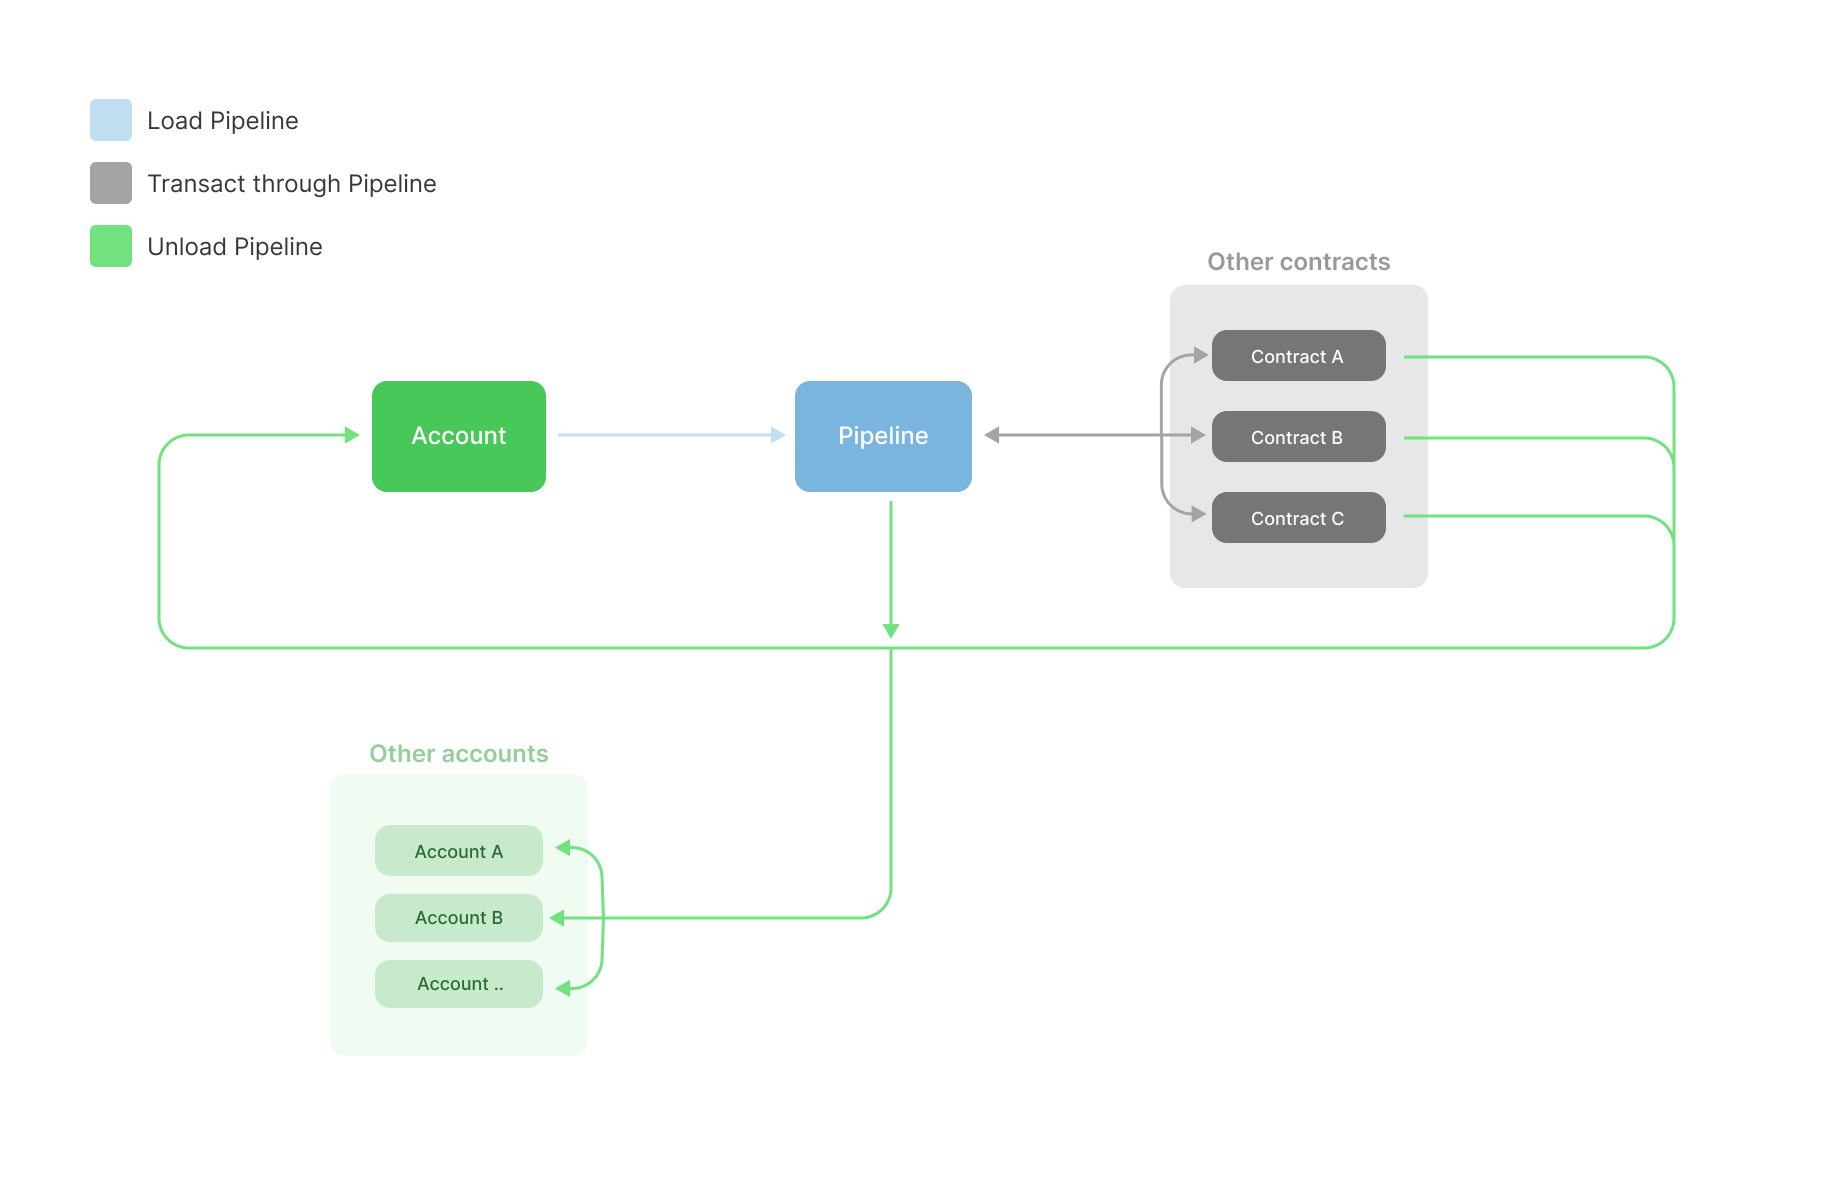
\includegraphics[scale=.65]{Figure1}
    \vspace*{-5mm}
    \caption{Using Pipeline}
    \label{fig 1}
\end{figure}

\newpage
\subsection{PipeCalls}
\term{PipeCalls} specify a function call to be executed by \term{Pipeline}. \term{Pipeline} supports 2 types of \term{PipeCalls}: \term{PipeCall} and \term{AdvancedPipeCall}.

\begin{enumerate}
    \item \textbf{\term{PipeCall}:} \term{PipeCall} makes a function call with a static target address and \code{callData}.
    \begin{lstlisting}[language=Solidity]
    struct PipeCall {
        address target;
        bytes data;
    }
    \end{lstlisting}

    \item \textbf{\term{AdvancedPipeCall}:} \term{AdvancedPipeCall} makes a function call with a static target address and both static and dynamic \code{callData}.
    \begin{lstlisting}[language=Solidity]
    struct AdvancedPipeCall {
        address target;
        bytes data;
        bytes clipboard; // See Section 5
    }
    \end{lstlisting}

\end{enumerate}

\subsection{Pipe Functions}
\term{Pipeline's} \term{Pipe} functions execute one or more \term{PipeCalls} or \term{AdvancedPipeCalls}. \term{Pipeline} has 3 \term{Pipe} functions: \code{pipe}, \code{multiPipe} and \code{advancedPipe}

\begin{enumerate}
    \item \code{pipe}: \code{pipe} executes a single \term{PipeCall}.
    \begin{lstlisting}[language=Solidity]
    function pipe(PipeCall calldata p)
        external
        payable
        returns (bytes memory result);
    \end{lstlisting}
    \item \code{multiPipe}: \code{multiPipe} executes a list of \term{PipeCalls}.
    \begin{lstlisting}[language=Solidity]
    function multiPipe(PipeCall[] calldata pipes)
        external
        payable
        returns (bytes[] memory results);
    \end{lstlisting}
    \item \code{advancedPipe}: \code{advancedPipe} executes a list of \term{AdvancedPipeCalls}.
    \begin{lstlisting}[language=Solidity]
    function advancedPipe(AdvancedPipeCall[] calldata pipes)
        external
        payable
        returns (bytes[] memory results);
    \end{lstlisting}
\end{enumerate}

\newpage
\section{Depot}
\term{Depot} wraps \term{Pipeline's} \term{Pipe} functions to facilitate the loading of non-Ether assets in \term{Pipeline} in the same transaction that loads Ether, \term{Pipes} calls to other protocols, and unloads \term{Pipeline}.

\term{Depot} has four functions that wrap \term{Pipeline's} \term{Pipe} functions.

\begin{enumerate}
    \item \code{pipe}: \code{pipe} wraps \term{Pipeline's} \code{pipe} function but does not support sending Ether.
    \begin{lstlisting}[language=Solidity]
    function pipe(PipeCall calldata p)
        external
        payable
        returns (bytes memory result);
    \end{lstlisting}
    \item \code{etherPipe}: \code{etherPipe} wraps \term{Pipeline's} \code{pipe} function and supports sending Ether.
    \begin{lstlisting}[language=Solidity]
    function etherPipe(PipeCall calldata p, uint256 value)
        external
        payable
        returns (bytes memory result);
    \end{lstlisting}
    \item \code{multiPipe}: \code{multiPipe} wraps \term{Pipeline's} \code{multiPipe} function but does not support sending Ether.
    \begin{lstlisting}[language=Solidity]
    function multiPipe(PipeCall[] calldata pipes)
        external
        payable
        returns (bytes[] memory results);
    \end{lstlisting}
    \item \code{advancedPipe}: \code{advancedPipe} wraps \term{Pipeline's} \code{advancedPipe} function and supports sending Ether.
    \begin{lstlisting}[language=Solidity]
    function advancedPipe(AdvancedPipeCall[] calldata pipes, uint256 value)
        external
        payable
        returns (bytes[] memory results);
    \end{lstlisting}
\end{enumerate}

\section{Clipboard}
\term{Clipboard} allows users to \term{Copy} return values stored as \code{returnData} from any \term{AdvancedPipeCalls} that have already been executed and \term{Paste} them into the \code{callData} of the next \term{AdvancedPipeCall}, in a customizable manner. 

Each \term{AdvancedPipeCall} includes \term{Clipboard} to encode (1) how many paste operations to perform, (2) which \code{returnData} from previous \term{AdvancedPipeCalls} to \term{Copy} (\term{i.e.}, \code{returnDataIndex}), (3) where to \term{Copy} from within (2) (\term{i.e.}, \code{copyIndex}), and (4) where to \term{Paste} it in the \code{callData} of the next \term{AdvancedPipeCall} (\term{i.e.}, \code{pasteIndex}). Bytes are \term{Pasted} 32 bytes at a time.

\term{Clipboard} defines a \code{Type}, whether to use Ether and how much, and corresponding \code{pasteParam(s)}, if necessary, for each \term{AdvancedPipeCall}.

\newpage
\subsection{Type}
The first byte of \term{Clipboard} defines its \code{Type}, which specifies the amount of \term{Pasting} operations in the \term{AdvancedPipeCall}. The \code{Type} is either \code{0x00}, \code{0x01} or \code{0x02}.

\begin{itemize}
    \item \textbf{\code{0x00} - Basic function call:} no bytes are \term{Pasted} (\term{i.e.}, a static function call).
    \item \textbf{\code{0x01} - 1 \code{bytes32} \term{Pasting} operation:} 1 \code{bytes32} is \term{Pasted} from a previous \term{AdvancedPipeCall's} \code{returnData}. 1 \code{pasteParams} are the first 32 bytes of the \term{Clipboard}.
    \item \textbf{\code{0x02} - n \code{bytes32} \term{Pasting} operations:} n \code{bytes32} are \term{Pasted} from previous \term{AdvancedPipeCalls'} \code{returnData}. Bytes 3 through 31 are left empty. Bytes 32 through 32 * (n + 2) are a \code{bytes32[]}, where each \code{bytes32} are the \code{pasteParams} for a given byte \term{Paste} operation.
\end{itemize}

\subsection{Ether Usage}
The second byte of \term{Clipboard} defines the \code{Use Ether Flag}, which specifies whether to include Ether in the \term{AdvancedPipeCall}. The \code{Use Ether Flag} is either \code{0x00} or \code{0x01}.

\begin{itemize}
    \item \textbf{\code{0x00}} - Do not send Ether in the \term{AdvancedPipeCall}.
    \item \textbf{\code{0x01}} - Send Ether in the \term{AdvancedPipeCall}. The amount of Ether to send is added as a \code{uint256} at the end of \term{Clipboard}.
\end{itemize}

\subsection{pasteParams}
\term{Clipboard} \code{Types} \code{0x01} and \code{0x02} accept one or more \code{pasteParams}, respectively, as inputs that encode where to \term{Copy} from, what to \term{Copy}, and where to \term{Paste} to, 32 bytes per \code{pasteParams}. 

\begin{itemize}
    \item \code{Empty} - bytes 0 - 1 are reserved for the Type and \code{Use Ether Flag}.
    \item \code{returnDataIndex} - bytes 2 - 11 specify the index of the \code{returnData} to \term{Copy} in the list of \code{returnData} from previously executed \term{AdvancedPipeCalls} in the current \code{advancedPipe} function call, ordered by execution (\term{e.g.}, \code{0x0000000000} \term{Copies} the \code{returnData} of the 0th \term{AdvancedPipeCall}, \code{0x0000000001} \term{Copies} the \code{returnData} of the 1st, etc.).
    \item \code{copyIndex} - bytes 12 - 21 specify the byte index in the corresponding \code{returnData[returnDataIndex]} to \term{Copy}. The first 32 bytes are the length of the return value (\term{e.g.}, \code{0x0000000020} \term{Copies} the 0th return value from \code{returnData[returnDataIndex]}, \code{0x0000000040} \term{Copies} the 1st return value, etc.).
    \item \code{pasteIndex} - bytes 22 - 31 specify the byte index of where to \term{Paste} onto the \code{callData} of the next \term{AdvancedPipeCall} (\term{e.g.}, \code{0x0000000024} \term{Pastes} onto the 0th parameter of the next \term{AdvancedPipeCall's} \code{callData}, \code{0x0000000044} \term{Pastes} onto the 1st parameter, etc.). 
\end{itemize}

\begin{figure}[h!]
    \centering
    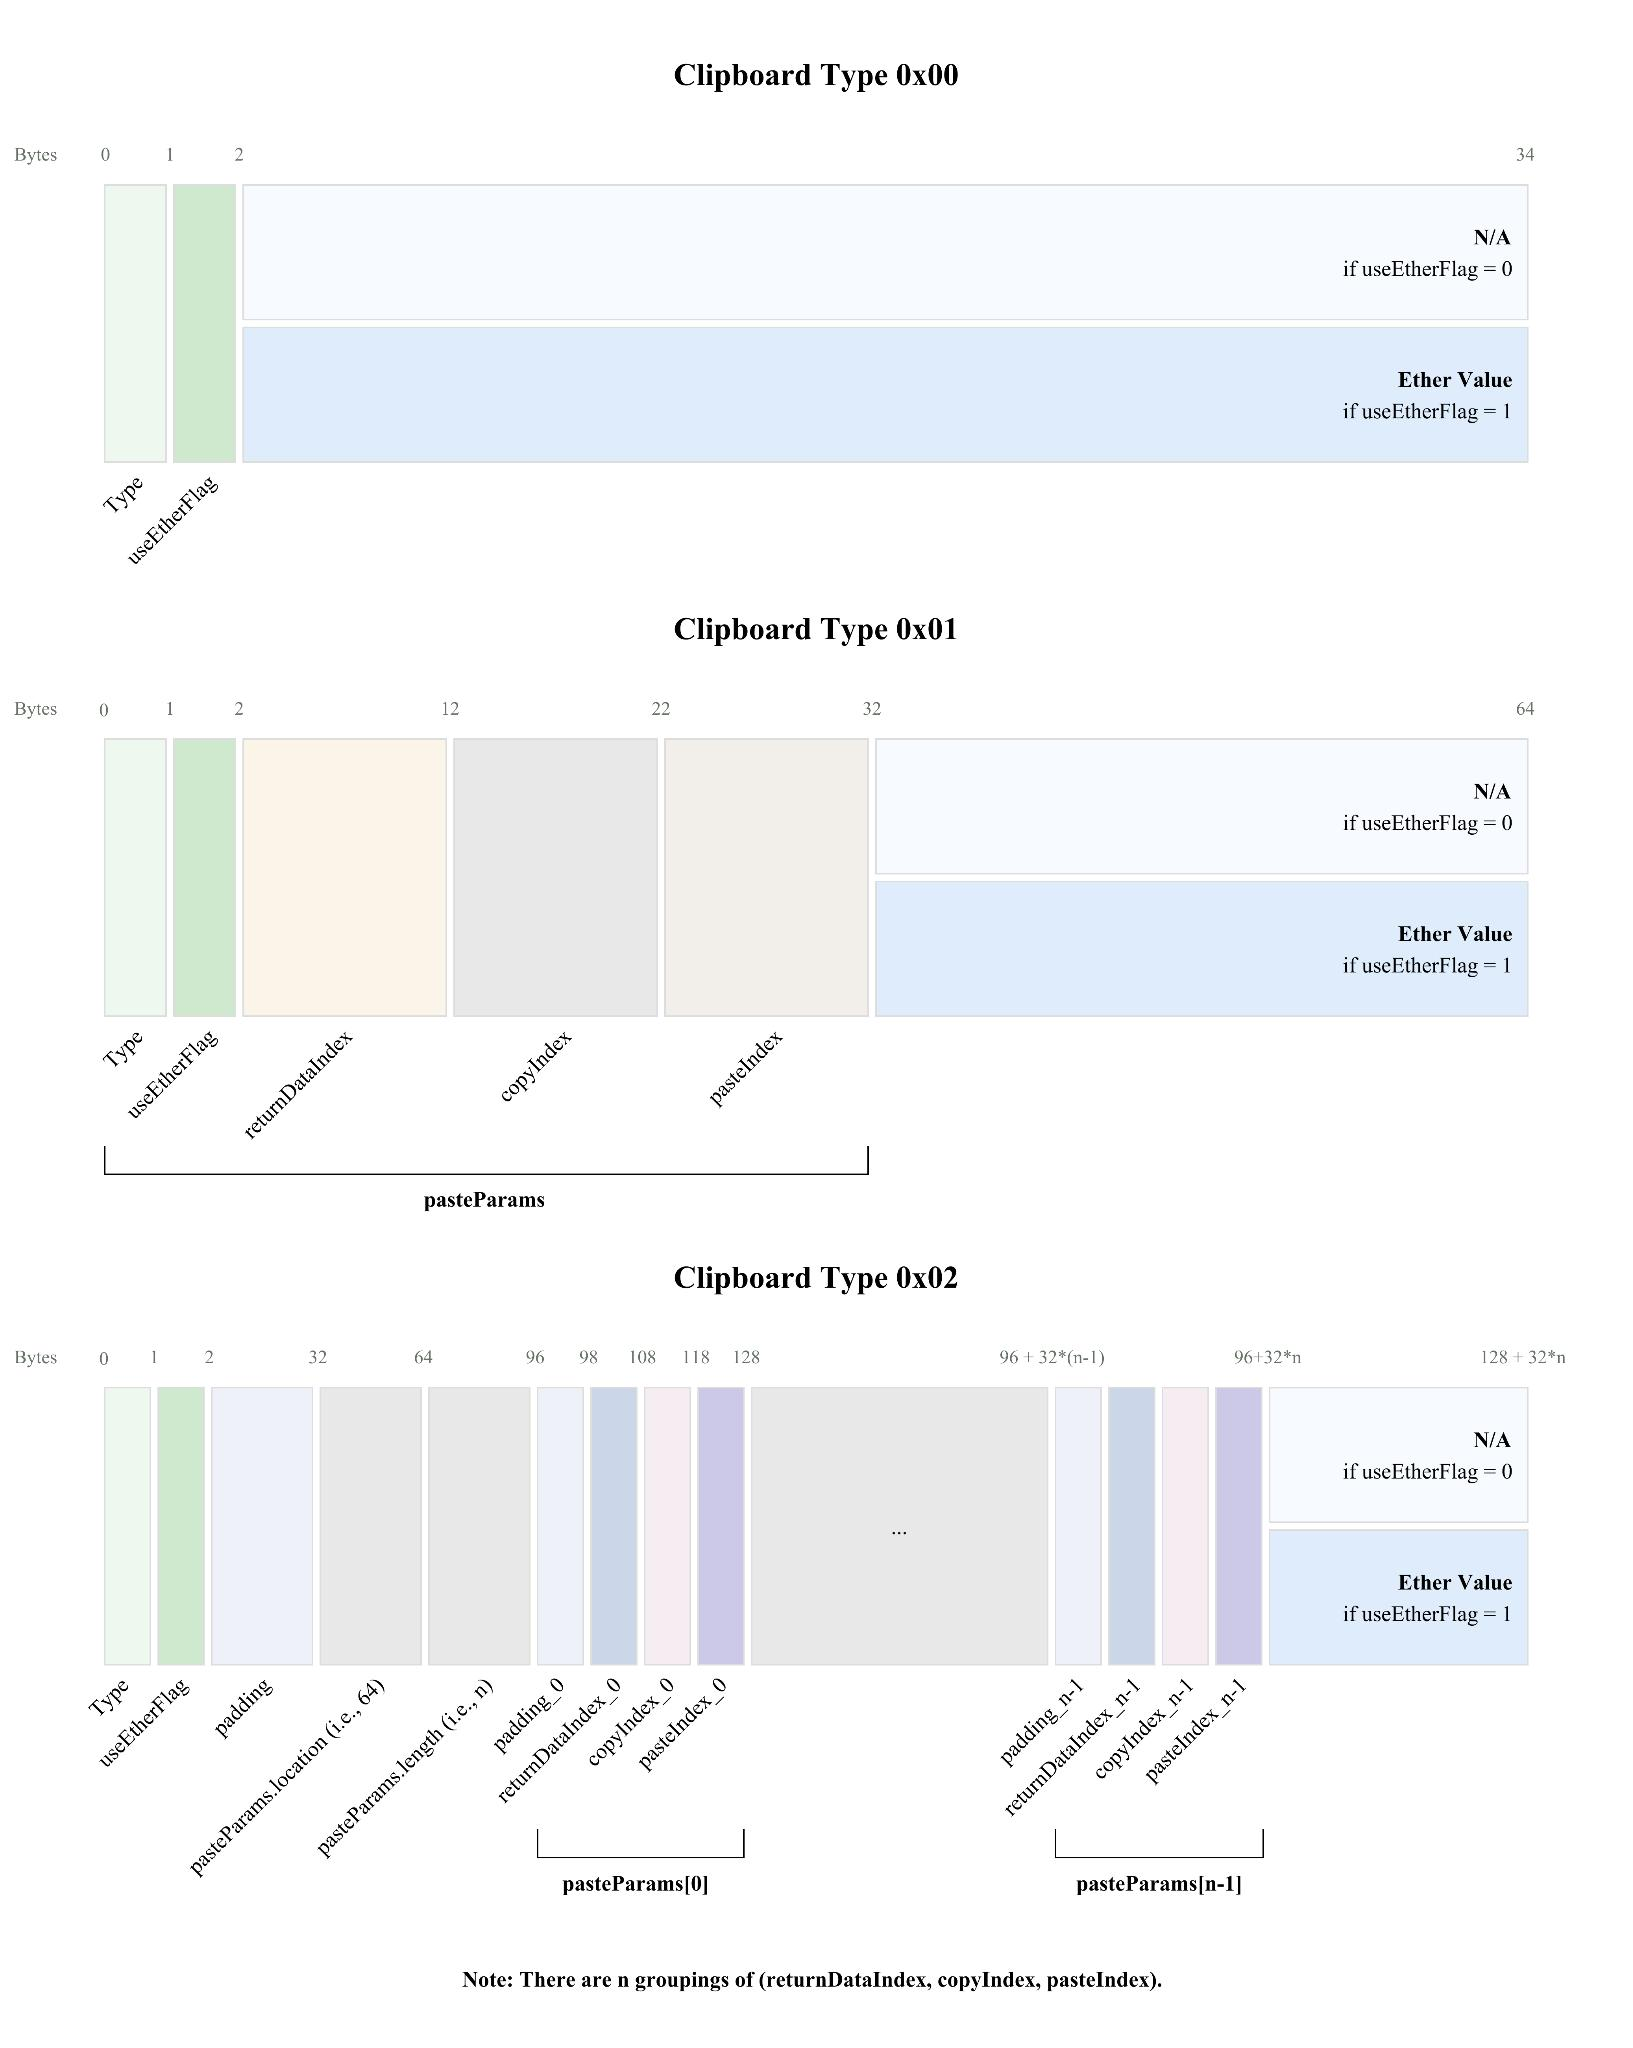
\includegraphics[scale=.89]{Figure2}
    % \vspace*{-5mm}
    \caption{Clipboard}
    \label{fig 2}
\end{figure}

\newpage
\section{Risk}
There are numerous risks associated with \term{Pipeline} and \term{Depot}. This is not an exhaustive list.

The \term{Pipeline}, \term{Depot} and \term{Clipboard} code bases are novel. None have been tested in the “real world” prior to their initial deployment. The open source nature of \term{Pipeline} and \term{Depot} means that others can take advantage of any bugs, flaws or deficiencies in them.

The majority of known risks associated with \term{Pipeline} are from misuse:

\begin{itemize}
    \item Failure to unload assets from \term{Pipeline} in the same transaction that loads it will highly likely result in a loss of those assets;
    \item Approving \term{Pipeline} to use any assets will highly likely result in a loss of those assets; and
    \item Improper encoding of \term{Clipboard} can result in a loss of funds or value. The complexity of properly encoding and decoding \term{Clipboard} makes verifying correctness difficult. 
\end{itemize}

\section{Future Work}
\term{Pipeline}, \term{Depot} and \term{Clipboard} are a work in progress. While \term{Pipeline} and \term{Depot} are non-upgradable, they can be easily forked and improved. The following are potential improvements that can be incorporated into them:

\begin{itemize}
    \item \term{Depot} easily can be further generalized to include other transferable asset types.
    \item Currently \term{Clipboard} only supports \term{Copying} 32 bytes at a time. Additional \term{Clipboard} \code{Types} can be added to allow the entry of an additional \code{copyLength} parameter.
    \item Tooling can be improved to make the encoding and decoding of \term{Clipboard} easier and more accessible.
    \item The ability to execute \term{PipeCalls} on various “layers” of the Ethereum network in a single transaction can be implemented.
\end{itemize}

\newpage
\section{Appendix}
\documentclass[class=article, crop=false]{standalone}
\usepackage[subpreambles=true]{standalone}
\usepackage{import}
\usepackage{enumitem} % Format list spacing 

\begin{document}

\subsection{Glossary}
The following terms are used throughout this Whitepaper:
\begin{itemize}[topsep=0pt, itemsep=3pt,leftmargin=16pt]
    \item[] \term{AdvancedPipeCall} - A type of \term{Pipecall} that makes a function call with a  static taget address and both static and dynamic \code{callData};
    \item[] \term{Clipboard} - A framework to \term{Copy} return values stored as \code{returnData} from any \term{AdvancedPipeCalls} that have already been executed and \term{Paste} them into the \code{callData} of the next \term{AdvancedPipeCall}, in a customizable manner;
    \item[] \term{Copy} - Add \code{bytes32 pasteParams} to the \term{Clipboard};
    \item[] \term{Deposit} - Assets in the \term{Silo};
    \item[] \term{Depot} - A wrapper for \term{Pipeline} that supports (1) loading Ether and non-Ether assets into \term{Pipeline}, (2) using them and (3) unloading them from \term{Pipeline}, in a single transaction;
    \item[] \term{Farm} - Where Beanstalk \term{Farm} balances are stored; 
    \item[] \term{Paste} - Add \code{bytes32 pasteParams} from the \term{Clipboard} to \code{callData} of the next \term{AdvancedPipeCall} to be executed;
    \item[] \term{Pipe} - \term{Pipeline's} functions that execute one or more \term{PipeCalls} or \term{AdvancedPipeCalls};
    \item[] \term{PipeCall} - A struct that specifies a function call to be executed by \term{Pipeline}. 
    \item[] \term{Pipeline} - A standalone contract that creates a sandbox to execute an arbitrary composition of valid actions within the EVM in a single transaction using Ether; and
    \item[] \term{Silo} - The Beanstalk DAO.
\end{itemize}
\end{document} % Glossary

\newpage
\documentclass[class=article, crop=false]{standalone}
\usepackage[subpreambles=true]{standalone}
\usepackage{import}
\usepackage{enumitem} % Format list spacing 

\begin{document}

\subsection{Whitepaper Version History}
The following is a complete version history of this whitepaper. Unless otherwise noted, references within this Whitepaper Version History are not updated to reflect later changes.

\begin{itemize}[topsep=0pt, itemsep=3pt,leftmargin=16pt]
    \item \href{https://github.com/BeanstalkFarms/Pipeline-Whitepaper/blob/master/version-history/pipeline1_0_0.pdf}{1.0.0} (November 16, 2022)
    \begin{itemize}
        \item Original Whitepaper.
    \end{itemize}
    \item \href{https://github.com/BeanstalkFarms/Pipeline-Whitepaper/blob/master/version-history/pipeline1_0_1.pdf}{1.0.1} (November 26, 2022)
    \begin{itemize}
        \item Corrected the link to the \href{https://github.com/BeanstalkFarms/Pipeline}{Pipeline GitHub Repository}.
        \item Corrected a typo in the second paragraph of \hyperlink{section.5}{Section 5}.
        \item Corrected the numbering in the second paragraph of \hyperlink{section.5}{Section 5}.
        \item Moved the \hyperlink{subsection.8.1}{Glossary} to \hyperlink{subsection.8.1}{Section 8.1} under \hyperlink{section.8}{Appendix}.
        \item Changed paper to Whitepaper in the intro to the \hyperlink{subsection.8.1}{Glossary}.
    \end{itemize}
    \item \href{https://github.com/BeanstalkFarms/Pipeline-Whitepaper/blob/master/version-history/pipeline1_0_2.pdf}{1.0.2} (May 25, 2023)
    \begin{itemize}
        \item Corrected a typo in the \term{AdvancedPipeCall} area of \hyperlink{subsection.3.2}{Section 3.2}.
    \end{itemize}
    \item \href{https://github.com/BeanstalkFarms/Pipeline-Whitepaper/blob/master/version-history/pipeline1_0_3.pdf}{1.0.3} (August 24, 2023)
    \begin{itemize}
        \item Updated Silo Chad's email address. 
    \end{itemize}
    \item \href{https://github.com/BeanstalkFarms/Pipeline-Whitepaper/blob/master/version-history/pipeline1_0_4.pdf}{1.0.4} (November 17, 2023)
    \begin{itemize}
        \item Corrected typos in \hyperlink{subsection.3.2}{Sections 3.2} and \hyperlink{subsection.5.2}{5.2}.
        \item Removed the second paragraph of \hyperlink{subsection.5.2}{Section 5.2}.
        \item Corrected a typo in the second paragraph of \hyperlink{section.6}{Section 6}.
        \item Changed Whitepaper to whitepaper in the intro to the Glossary.
    \end{itemize}
    
\end{itemize}
\end{document} % Whitepaper Version History 

\end{document}